\documentclass[border=4pt]{standalone}

\usepackage{tikz}

\definecolor{otblue}{HTML}{0072B2}
\definecolor{otorange}{HTML}{E69F00}
\definecolor{otteal}{HTML}{009E73}
\definecolor{otpurple}{HTML}{CC79A7}
\definecolor{otgray}{HTML}{5A5A5A}

\begin{document}
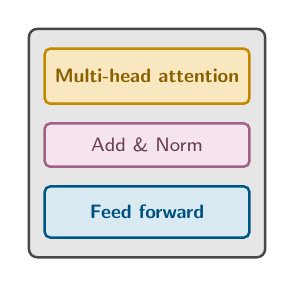
\begin{tikzpicture}[line width=0.9pt]
  \filldraw[draw=otgray!80!black, fill=otgray!15, rounded corners=3pt] (0,0) rectangle (3,2.9);
  \filldraw[draw=otorange!85!black, fill=otorange!25, rounded corners=2pt] (0.2,1.95) rectangle (2.8,2.65);
  \node[font=\sffamily\scriptsize\bfseries, text=otorange!60!black] at (1.5,2.3) {Multi-head attention};
  \filldraw[draw=otpurple!80!black, fill=otpurple!20, rounded corners=2pt] (0.2,1.15) rectangle (2.8,1.7);
  \node[font=\sffamily\scriptsize, text=otpurple!50!black] at (1.5,1.425) {Add \& Norm};
  \filldraw[draw=otblue!75!black, fill=otblue!15, rounded corners=2pt] (0.2,0.25) rectangle (2.8,0.9);
  \node[font=\sffamily\scriptsize\bfseries, text=otblue!70!black] at (1.5,0.575) {Feed forward};
\end{tikzpicture}
\end{document}
